\documentclass{article}
\usepackage[legalpaper, margin=1in]{geometry}
\usepackage[utf8]{inputenc}
\usepackage{hyperref}
\usepackage{graphicx}
\usepackage{amsmath,amssymb,amsfonts}
\usepackage{float}
\usepackage{listings}
\usepackage{minted}
\usepackage{xcolor}
\usepackage{pifont}% http://ctan.org/pkg/pifont
\newcommand{\cmark}{\ding{51}}%
\newcommand{\xmark}{\ding{55}}%
\usepackage{caption}
\definecolor{LightGray}{gray}{0.9}
\setminted{
	linenos=true,
	autogobble,
}

\hypersetup{
	colorlinks   = true, %Colours links instead of ugly boxes
	urlcolor     = blue, %Colour for external hyperlinks
	linkcolor    = blue, %Colour of internal links
	citecolor   = red %Colour of citations
}

\title{Formal Semantics}
\author{}
\date{}

\begin{document}
\maketitle

\section{Defining Concrete Examples}

\begin{figure}[H]
	\caption{Example Robot 1}
	\centering
	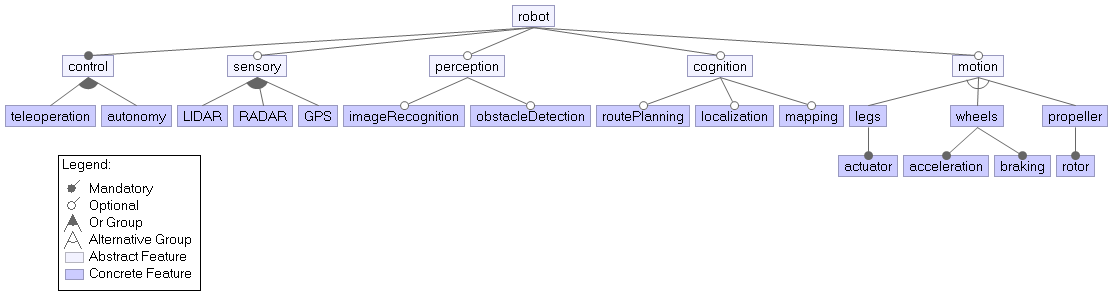
\includegraphics[width=0.99\textwidth]{images/exp.png}
	\label{conmet}
\end{figure}

\begin{table}[H]
	\caption{Allowed Binding Times and Modes For Figure \ref{conmet}}
	\centering
	\begin{center}
		\begin{tabular}{c c c c c c}
			\hline
			Feature & Property & Static Early (SE) & Static Late (SL) & Dynamic Early (DE) & Dynamic Late (DL) \\\hline
			robot(root) & Mandatory & \checkmark & \xmark & \xmark & \xmark \\ \hline
			control & Mandatory & \checkmark & \checkmark & \xmark & \xmark \\ \hline
			sensory & Optional & \checkmark & \xmark & \xmark & \xmark \\ \hline
			perception & Optional & \checkmark & \xmark & \xmark & \xmark \\ \hline
			cognition & Optional & \checkmark & \xmark & \xmark & \xmark \\ \hline
			motion & Optional & \checkmark & \xmark & \xmark & \xmark \\ \hline
			teleoperation & OR & \checkmark & \checkmark & \checkmark & \checkmark \\ \hline
			autonomy & OR  & \checkmark & \checkmark & \checkmark & \checkmark \\ \hline
			LIDAR & OR  & \checkmark & \checkmark & \checkmark & \checkmark \\ \hline
			RADAR & OR  & \checkmark & \checkmark & \checkmark & \checkmark \\ \hline
			GPS & OR  & \checkmark & \checkmark & \checkmark & \checkmark \\ \hline
			imageRecognition & Optional & \xmark & \xmark & \checkmark & \checkmark \\ \hline
			obstacleDetection & Optional & \xmark & \xmark & \checkmark & \checkmark \\ \hline
			routePlanning & Optional & \xmark & \xmark & \checkmark & \checkmark \\ \hline
			localization & Optional & \xmark & \xmark & \checkmark & \checkmark \\ \hline
			mapping & Optional & \xmark & \xmark & \checkmark & \checkmark \\ \hline
			legs & XOR &\xmark & \xmark & \checkmark & \checkmark \\ \hline
			actuator & Mandatory & \checkmark & \checkmark & \xmark & \xmark \\ \hline
			wheels & XOR & \xmark & \xmark & \checkmark & \checkmark \\ \hline
			acceleration & Mandatory & \checkmark & \checkmark & \xmark & \xmark \\ \hline
			braking & Mandatory & \checkmark & \checkmark & \xmark & \xmark \\ \hline
			propeller & XOR & \xmark & \xmark & \checkmark & \checkmark \\ \hline
			rotor& Mandatory & \checkmark & \checkmark & \xmark & \xmark \\ \hline
			
		\end{tabular}
		\label{tab:rob1}
	\end{center}
\end{table}


\begin{figure}[H]
	\caption{Example Robot 2}
	\centering
	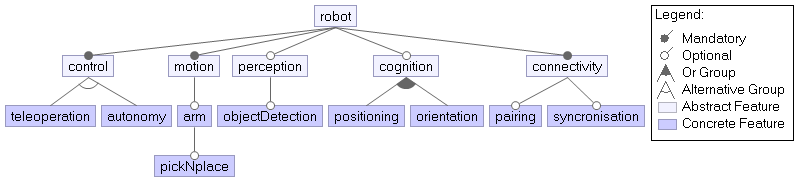
\includegraphics[width=0.99\textwidth]{images/robo2.png}
	\label{robo2}
\end{figure}

\begin{table}[H]
	\caption{Allowed Binding Times and Modes For Figure \ref{robo2}}
	\centering
	\begin{center}
		\begin{tabular}{c c c c c c}
			\hline
			Feature & Property & Static Early (SE) & Static Late (SL) & Dynamic Early (DE) & Dynamic Late (DL) \\\hline
			robot(root) & Mandatory & \checkmark & \xmark & \xmark & \xmark \\ \hline
			control & Mandatory & \checkmark & \checkmark & \xmark & \xmark \\ \hline
			motion & Mandatory & \checkmark & \checkmark & \xmark & \xmark \\ \hline
			perception & Optional & \checkmark & \xmark & \xmark & \xmark \\ \hline
			cognition & Optional & \checkmark & \xmark & \xmark & \xmark \\ \hline
			connectivity & Mandatory & \checkmark & \checkmark & \xmark & \xmark \\ \hline
			pairing & Optional & \xmark & \xmark & \checkmark & \checkmark \\ \hline
			synchronisation & Optional & \xmark & \xmark & \checkmark & \checkmark \\ \hline
			positioning & OR & \checkmark & \checkmark & \checkmark & \checkmark \\ \hline
			orientation & OR & \checkmark & \checkmark & \checkmark & \checkmark \\ \hline
			objectDetection & Optional & \xmark & \xmark & \checkmark & \checkmark \\ \hline
			arm & Optional & \xmark & \xmark & \checkmark & \checkmark \\ \hline
			pickNplace & Optional & \xmark & \xmark & \checkmark & \checkmark \\ \hline
			teleoperation & XOR & \xmark & \xmark & \checkmark & \checkmark \\ \hline
			autonomy & XOR & \xmark & \xmark & \checkmark & \checkmark \\ \hline
		\end{tabular}
		\label{tab:tabr2}
	\end{center}
\end{table}

\section{Deducing General Language Semantics}

For any given feature pairs represented arbitrarily by A and B, where A and B are objects of our meta-model i.e they can be assigned a binding time and binding mode value, the table below represents valid and invalid pairs of A and B that can exist under mandatory, optional, inclusion, exclusion, OR and  XOR constraints, for any given feature model. 1s denote that the pairing is valid while 0s denote that a corresponding pairing is invalid.

For example: 

\begin{table}[H]
	\caption{Feature Model Binding Semantics: \textbf{S = Static, E = Early, L = Late, D = Dynamic}}
	\centering
	\begin{center}
		\begin{tabular}{c c c c c c c c}
			\hline
			A & B & $ \neg$ B & A $ \Rightarrow $ $ \neg $ B & A $ \Rightarrow $ B & A $ \Leftrightarrow $ B & A $\vee$ B & A $\oplus$ B\\\hline
			SE & SE & DL & 0 & 1 & 1 & 1 & 0 \\ \hline
			SE & SL & DE & 0 & 0 & 0 & 1 & 0 \\ \hline
			SE & DE & SL & 0 & 0 & 0 & 1 & 0 \\ \hline
			SE & DL & SE & 1 & 0 & 0 & 1 & 0 \\ \hline
			
			SL & SE & DL & 0 & 1 & 0 & 1 & 0 \\ \hline 
			SL & SL & DE & 0 & 1 & 1 & 1 & 0 \\ \hline
			SL & DE & SL & 1 & 0 & 0 & 1 & 0 \\ \hline
			SL & DL & SE & 1 & 0 & 0 & 1 & 0 \\ \hline
			
			DE & SE & DL & 0 & 1 & 0 & 1 & 0 \\ \hline
			DE & SL & DE & 0 & 0 & 0 & 1 & 0 \\ \hline
			DE & DE & SL & 0 & 0 & 0 & 1 & 1 \\ \hline
			DE & DL & SE & 1 & 0 & 0 & 1 & 1 \\ \hline
			
			DL & SE & DL & 0 & 1 & 0 & 1 & 0\\ \hline
			DL & SL & DE & 0 & 1 & 0 & 1 & 0\\ \hline
			DL & DE & SL & 1 & 0 & 0 & 1 & 1 \\ \hline
			DL & DL & SE & 0 & 0 & 0 & 1 & 1 \\ \hline
			
		\end{tabular}
		\label{tab:timoconf}
	\end{center}
\end{table}

Using DNF, the following propositional logic formulas were generated from the table above.

\begin{itemize}
	\item \textit{\textbf{Mandatory:}}\\ (A $ \Leftrightarrow $ B) $\equiv$ (SE $\wedge$ SE) $\vee$ (SL $\wedge$ SL)
	\item \textit{\textbf{Optional:}}\\ (A $ \Rightarrow $ B) $\equiv$ (SE $\wedge$ SE) $\vee$ (SL $\wedge$ SE) $\vee$ (SL $\wedge$ SL) $\vee$ (DE $\wedge$ SE) $\vee$ (DL $\wedge$ SE) $\vee$ (DL $\wedge$ SL)
	\item \textit{\textbf{Inclusion:}}\\ (A $ \Rightarrow $ B) $\equiv$ (SE $\wedge$ SE) $\vee$ (SL $\wedge$ SE) $\vee$ (SL $\wedge$ SL) $\vee$ (DE $\wedge$ SE) $\vee$ (DL $\wedge$ SE) $\vee$ (DL $\wedge$ SL)
	\item \textit{\textbf{Exclusion:}}\\ (A $ \Rightarrow $ $ \neg $ B) $\equiv$ (SE $\wedge$ SE) $\vee$ (SL $\wedge$ SL) $\vee$ (SL $\wedge$ SE) $\vee$ (DE $\wedge$ SE) $\vee$ (DL $\wedge$ SL)
	\item \textit{\textbf{OR:}}\\ (A $ \vee $ B) $\equiv$ (SE $\wedge$ SE) $\vee$ (SE $\wedge$ SL) $\vee$ (SE $\wedge$ DE) $\vee$ (SE $\wedge$ DL) $\vee$ (SL $\wedge$ SE) $\vee$ (SL $\wedge$ SL) $\vee$ (SL $\wedge$ DE) $\vee$ (SL $\wedge$ DL) $\vee$ (DE $\wedge$ SE) $\vee$ (DE $\wedge$ SL) $\vee$ (DE $\wedge$ DE) $\vee$ (DE $\wedge$ DL) $\vee$ (DL $\wedge$ SE) $\vee$ (DL $\wedge$ SL) $\vee$ (DL $\wedge$ DE) $\vee$ (DL $\wedge$ DL)
	\item \textit{\textbf{XOR:}}\\ (A $ \oplus $ B) $\equiv$ (DE $\wedge$ DE) $\vee$ (DE $\wedge$ DL) $\vee$ (DL $\wedge$ DE) $\vee$ (DL $\wedge$ DL)
\end{itemize}

\end{document}



